\documentclass[fr]{../../../eplsummary}

\usepackage[SIunits]{../../../eplunits}
\usepackage{../../../eplcode}

\usepackage{graphicx}
\usepackage{caption}
\usepackage{subcaption}
\newcommand{\laplace}{\mathcal{L}}

\lstset{language=Matlab}

\newcommand{\sbt}{\,\begin{picture}(-1,1)(-1,-3)\circle*{2.5}\end{picture}\ }
\newcommand{\umin}{u_\mathrm{min}}
\newcommand{\umax}{u_\mathrm{max}}

\usepackage{tikz}
\usepackage{pgfplots}
\usetikzlibrary{arrows,calc}

\hypertitle{Automatique Linéaire}{6}{INMA}{1510}
{Benoît Legat}
{Denis Dochain}

% http://me.berkeley.edu/~maxchen/_static/block_diagram_in_latex.pdf
\tikzstyle{block} = [draw, rectangle, minimum height=2em, minimum width=4em]
%fill=blue!20
\tikzstyle{sum} = [draw, fill=blue!20, circle, node distance=1cm]
\tikzstyle{input} = [coordinate] \tikzstyle{output} = [coordinate]
\tikzstyle{pinstyle} = [pin edge={to-,thin,black}]

% Pour éviter d'avoir un zéro (s+a) dans Tr(s) car il dégrade la dynamique,
% prendre un précompensateur a/(s+a)
% Par exemple, on ne peut pas l'identifier avec w_n, xhi et 10wn.
% voir 6.1, 6.2, 8.1

% Si état observable/commandable, utiliser retour d'état !

% Bode phase et log module s'additionnent log(k0) = 0

\section{Règle de Mason}
Le principe est expliqué assez clairement dans \cite{chau2002mason}
avec des exemples pour illustrer.
En résumé, on considère le schéma bloc comme un graphe dirigé et
pour calculer la fonction de transfert entre $a$ et $b$.
On prend
\begin{itemize}
  \item tous les chaines directes $F_k$ (c'est des chemins pour prendre la vocable des graphes, ce qui signifie qu'on ne fait pas de cycle),
  \item toutes les boucles $\{L_i\}$ (les cycles dans le vocable des graphes),
  \item toutes les boucles qui ne touchent \emph{pas} $F_k$: $\{L_{k;i}\}$.
\end{itemize}
Et on a la fonction de transfert par la formule suivante
\[ H(s) = \frac{\sum_k F_k\Delta(\{L_{k;i}\})}{\Delta(\{L_i\})} \]
où
\[ \Delta(\{L_j\}) = 1 - \sum_{j_1} L_{j_1} + \sum_{j_1,j_2} L_{j_1}L_{j_2} - \sum_{j_1,j_2,j_3} L_{j_1}L_{j_2}L_{j_3} + \cdots \]
avec $j_1, j_2, \ldots, j_n$ tels que les boucles $L_{j_1}, L_{j_2}, \ldots, L_{j_n}$ ne se touchent \emph{pas}.
Si toutes les boucles, se touchent, ça devient donc simplement
\( 1 - \sum_{j_1} L_{j_1}. \)
On remarque que $\Delta(\emptyset) = 1$.
La plupart du temps, les chaines directes touchent toutes les boucles et le numérateur devient donc $\sum_k F_k$ car $\{F_{k;i}\} = \emptyset$.

\begin{myexem}
  \label{ex:masonex}
  Pour l'exemple de la \figuref{masonex}, on a
  \begin{itemize}
    \item deux chaines directes qui valent respectivement $A(s)C(s)$ et $A(s)D(s)$,
    \item deux boucles qui valent respectivement $-A(s)B(s)$ et $D(s)E(s)$,
    \item la première chaine directe ne touche que par la première boucle et la deuxième passe les touchent toutes.
  \end{itemize}
  On a donc, comme les deux boucles ne se touchent pas,
  \[ H(s) = \frac{A(s)C(s)(1 - D(s)E(s)) + A(s)D(s)}{1 + A(s)B(s) - D(s)E(s) - A(s)B(s)D(s)E(s)}. \]
  \begin{figure}[!ht]
    \centering
    \begin{tikzpicture}[auto, node distance=2cm,>=latex']
      \node [input, name=input] {};
      \node [sum, right of=input] (sum) {};
      \node [block, right of=sum, node distance=2cm] (A) {$A(s)$};
      \node [block, below of=A] (B) {$B(s)$};
      \node [block, right of=A, node distance=6cm] (C) {$C(s)$};
      \node [block, below of=C, node distance=2cm] (D) {$D(s)$};
      \node [block, below of=D, node distance=2cm] (E) {$E(s)$};
      \node [sum, right of=C, node distance=2cm] (sum2) {};
      \node [sum, left of=D, node distance=1.5cm] (sum3) {};
      \node [output, right of=sum2] (output) {};
      \draw [->] (input) -- node {$a(t)$} (sum);
      \draw [->] (A) -- node[name=Ar,pos=0.3] {} node[name=Cl,pos=0.7] {} (C);
      \draw [->] (Ar) |- (B);
      \draw [->] (B) -| node[pos=0.45] (Bl) {} node[pos=0.95] {$-$} (sum);
      \draw [->] (sum) -- (A);
      \draw [->] (Cl) |- (sum3);
      \draw [->] (sum3) -- (D);
      \draw [->] (C) -- (sum2);
      \draw [->] (D) -| node[pos=0.3] (Dr) {} (sum2);
      \draw [->] (Dr) |- (E);
      \draw [->] (E) -| (sum3);
      \draw [->] (sum2) -- node {$b(t)$} (output);
    \end{tikzpicture}
    \caption{Schéma-block de l'exemple~\ref{ex:masonex}.}
    \label{fig:masonex}
  \end{figure}
\end{myexem}

\section{Erreur statique}
L'erreur est définie par $r(t) - y(t)$.
L'erreur statique est $\lim_{t\to\infty} r(t) - y(t)$.
Seulement, on sait que pour tout signal $f$, $\lim_{t\to\infty} f(t) = \lim_{s \to 0} sF(s)$.
On a donc, par le principe de superposition,
une erreur de commande de
\[ \lim_{s \to 0} s(1 - T_r(s))R(s) \]
et une erreur de perturbation de
\[ \lim_{s \to 0} sT_v(s)V(s). \]

En se rappelant que $\laplace(u(t)) = \frac{1}{s}$\footnote{$u(t)$ est un échelon, pas la commande.},
que $\laplace(tu(t)) = \frac{1}{s^2}$
et que $\laplace(\sin(\omega_0 t)) = \frac{1}{s^2+\omega_0^2}$, on trouve que,
pour ne pas avoir d'erreur statique,
\begin{itemize}
  \item pour $r(t) = u(t)$, il faut que $CG$ ait un pôle nul,
    aussi appelée action intégrale $\frac{1}{s}$;
  \item pour $r(t) = t u(t)$, il faut que $CG$ ait un double pôle nul $\frac{1}{s^2}$;
  \item pour $r(t) = \sin(\omega_0 t)$ (ou $\cos$, c'est pareil), il faut que $CG$ ait les pôles conjugués $\frac{1}{s^2+\omega_k^2}$.
\end{itemize}
En effet, par exemple, pour $r(t) = u(t)$, on a
\begin{align*}
  \lim_{s \to 0} s\left(1 - \frac{\frac{1}{s}C_0(s)G(s)}{1+\frac{1}{s}C_0(s)G(s)}\right)\frac{1}{s}
  & = \lim_{s \to 0} 1 - \frac{C_0(s)G(s)}{s+C_0(s)G(s)}\\
  & = 1 - \frac{C_0(s)G(s)}{C_0(s)G(s)}\\
  & = 1 - 1\\
  & = 0.
\end{align*}

En résumé, si $G$ n'a pas déjà les pôles voulus et qu'il ne les a pas en zéros, prêt à nous annuler
nos pôles bien placés, pour avoir une erreur statique nulle avec
\[ r(t) = \alpha_0 + \alpha_1 t + \cdots + \alpha_q t^q + \sum_{k=1}^p \beta_k \sin(\omega_k t + \phi_k), \]
il suffit de prendre
\[ C(s) = \frac{1}{s^q} \prod_{k=1}^p \left(\frac{1}{s^2+\omega_k^2}\right) C_0(s) \]
où $C_0$ n'a évidemment pas des zéros où on a mis nos pôles.

\paragraph{Erreur statique nulle avec perturbation}
Pour ne pas avoir d'erreur statique,
\begin{itemize}
  \item pour $v(t) = u(t)$, il faut que $CG$ ait plus de pôles nuls que $H$.
    Si $H$ a un zéro nul, on a même pas besoin d'avoir de pôle nul et donc d'action intégrale.
\end{itemize}

\section{Nyquist}
Nyquist est un outil qui nous permet de trouver le nombre de zéros instables de
$1 + C(s)G(s)$ si on connait le nombre de pôle instables de $C(s)G(s)$ et
donc de déterminer si notre fonction de transfert avec $1+C(s)G(s)$ au dénominateur
est stable, c'est à dire qu'il n'y a aucun zéro instable.

Soit $C(s)G(s) = \frac{N(s)}{D(s)}$, on a $1 + C(s)G(s) = \frac{D(s)+N(s)}{D(s)}$.
Les pôles de $C(s)G(s)$ sont donc les mêmes que ceux de $1 + C(s)G(s)$.
Le théorème de Cauchy nous dit que si on prend un parcours fermé $\Gamma$,
\[ N = P - Z \]
où $N$ est le nombre de fois que $(1 + CG) \circ \Gamma$ tourne autours de l'origine dans le sens
trigonométrique et $P$ et $Z$ sont le nombre de pôles et de zéros qui sont dans
le contour (on ne peut pas l'appliquer s'il y en a sur le contour).

\begin{figure}
  \centering
  \begin{subfigure}{0.49\linewidth}
    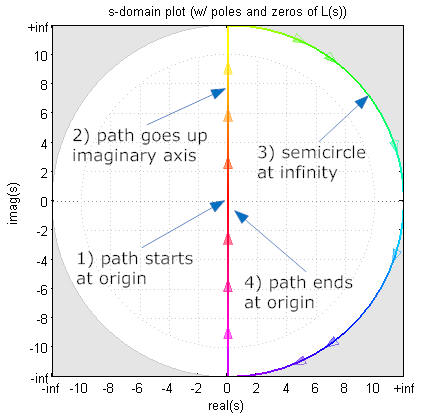
\includegraphics[width=\linewidth,height=\linewidth]{nyquistpath.jpg}
    \caption{Courbe fermée regroupant les racines instables.}
    \label{fig:nyquistpath}
  \end{subfigure}
  \begin{subfigure}{0.49\linewidth}
    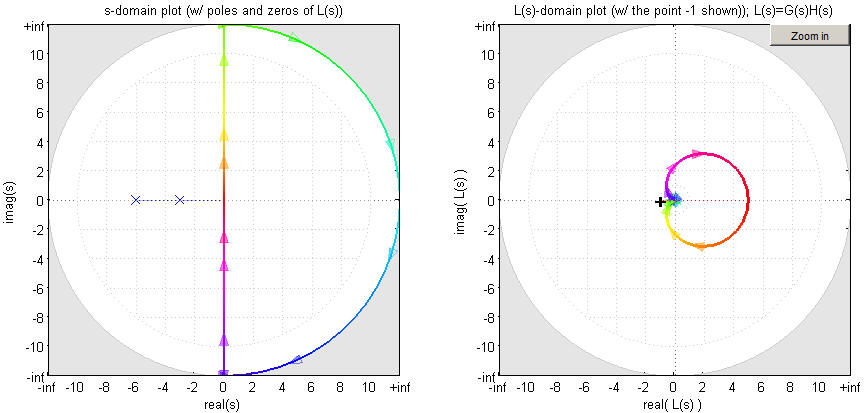
\includegraphics[trim=22cm 0cm 0cm 0cm,clip,width=\linewidth,height=\linewidth]{nyquistplot.jpg}
    \caption{Image de la courbe par $C(s)G(s)=\frac{90}{(s+3)(s+6)}$.}
    \label{fig:nyquistplot}
  \end{subfigure}
  \caption{Exemple de diagramme de Nyquist~\cite{cheever2013nyquist}.}
  \label{fig:nyquist}
\end{figure}

\begin{figure}
  \centering
  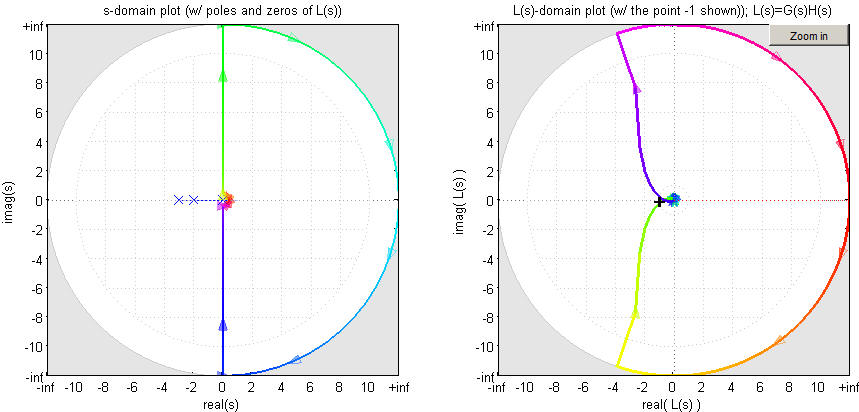
\includegraphics[width=\linewidth,height=0.45\linewidth]{nyquistint.jpg}
  \caption{Diagramme de Nyquist pour une fonction de transfert
  avec action intégrale~\cite{cheever2013nyquist}.}
  \label{fig:nyquistint}
\end{figure}


Si on prend le coutour de la \figuref{nyquistpath},
on regroupe donc toutes les racines instables.
Si on connait le nombre de pôles instables de $CG$, on a $P$ et ce qu'on cherche,
$Z$ est simplement $P - N$.
Si $CG$ a des racines ou pôles sur l'axe imaginaire, on ne peut pas appliquer le
critère car ils sont sur le contour, c'est problématique car on a souvent un
pôle nul avec l'action intégrale.
La solution est de passer par un petit demi-cercle de rayon $\epsilon$ autour
de 0 comme fait à la \figuref{nyquistint}.
Pour ce cours, on ne s'en soucie pas trop.
\cite{cheever2013nyquist} apporte de plus amples informations à ce sujet.

Au lieu de plotter $1 + CG$ et de regarder combien de fois on tourne autour
de l'origine,
on va plotter $CG$ et regarder combien de fois on tourne autour de $-1 + 0j$
ce qui revient au même.
On obtient alors un graphe semblable à la \figuref{nyquistplot}.

Pour trouver $N$, il suffit de prendre une demi-droite partant de $-1$ et
allant à l'infini dans n'importe quel sens, à chaque fois qu'on rencontre
la courbe, si elle va vers la gauche, on fait $+1$, sinon, on fait $-1$.
Au final, on aura $N$ (c'est bien illustré par \cite{cheever2013nyquist}).

\subsection{Allure classique}
Au final, on a souvent $P = 0$ et $CG$ a souvent soit des pôles ou racines
conjuguées, soit des pôles ou racines réelles négatives, soit un pôle
nul dû à l'action intégrale.
Nos pôles et racines sont toujours avec leur conjuguées car on a des coefficients
réels dans nos polynômes.

Dans le parcours de la \figuref{nyquistpath}, on traverse la droite
$s = j\omega$ de $\omega = -\infty$ à $\omega = \infty$ en passant par $\omega = 0$
(ou plutôt en faisant un demi-cercle de rayon $\epsilon$ autour si on a une action intégrale).
En $\omega = 0$, la phase de $CG$ est soit 0 comme pour la \figuref{nyquistplot},
soit $-\ang{90}$ en $\epsilon$ et $\ang{90}$ en $-\epsilon$ si on a une action intégrale.
En effet la phase est la somme des phase des différents facteurs.
\begin{itemize}
  \item
    Pour les racines et pôles réels positifs, on a $s + r_i$ avec $r_i > 0$ donc
    pour $s = 0$, on a une phase nulle.
  \item
    Pour les racines et pôles conjuguées, ils ont des phases opposées donc leur somme
    est nulle.
  \item
    L'action intégrale a la phase de $\frac{1}{\epsilon j} = -\frac{1}{\epsilon} j \to -\infty j$
    qui a un module infini et une phase de $-\ang{90}$ pour $\omega = \epsilon$.
    Le module infini explique pourquoi on vient souvent de $-\infty j$ quand on a une action
    intégrale.
    C'est ce qu'on voit sur la \figuref{nyquistint} où la phase n'est pas exactement
    $-\ang{90}$ car pour les pôles réels positif, on a $j\epsilon + r_i$ et pas juste $r_i$.
\end{itemize}

Si $CG$ est strictement propre (le degré du dénominateur est plus grand que celui du dénominateur),
lorsque $|\omega| \to \infty$, le module de $CG$ tend vers 0, on passe donc par l'origine comme
le montre la \figuref{nyquistplot}.

Comme on a supposé que $CG$ n'a pas de pôles instables, $P = 0$ et donc $Z = -N$.
Il faut donc que $N = 0$ pour avoir un système stable.

Comme nos polynômes sont à coefficients réels,
$C(-j\omega)G(-j\omega) = C(\bar{j\omega})G(\bar{j\omega}) = \bar{C(j\omega)G(j\omega)}$.
On fait donc le même trajet pour $\omega$ allant de $-\infty$ à $0$ qu'on a fait
pour $\omega$ allant de $0$ à $\infty$ mais dans l'autre sens et de l'autre côté de l'axe réel.
C'est exactement ce qu'on voit à la figure \figuref{nyquistplot}.

S'il n'y a pas d'action intégrale, la partie de la courbe de $\omega = 0$ à $\omega = \infty$
part donc de $C(0)G(0)$ qui est un réel positif
et abouti en $0$ si $CG$ est strictement propre, comme on a vu, on fait après exactement pareil
de l'autre côté de l'axe réel.
Avec action intégrale, on part de $-\infty j$ et on abouti en $0$ puis on fait pareil
mais vers $\infty j$ puis pendant qu'on fait notre petit demi-cerce de rayon $\epsilon$ autour
de l'origine, on passe de $\infty j$ à $-\infty j$ par la droite (parce que).

On peut donc juste regarder ce qu'on fait de $\omega = 0$ à $\omega = \infty$.
Si on passe à gauche du point $-1$,
alors on fera un tour dans le sens horlogique et donc
$N = -1$ ce qui fait $Z = 1$, on est donc instable.
Si on y passe à droite, alors $N = 0$ et donc $Z = 0$ et on est stable!

\section{Root Locus}
On appelle ``Root Locus'', la location des racines du polynômes caractéristique
(le dénominateur de $T_r$ et $T_v$) en fonction d'un gain $k_0$ tel que $C(s) = k_0C_0(s)$.
Soit $\frac{N(s)}{D(s)} \eqdef = C_0(s)G(s)$, le polynôme caractéristique vaut $D(s) + kN(s)$.
Soient $n \eqdef \deg(D)$ et $m \eqdef \deg(N)$.
\begin{itemize}
  \item Pour $k_0 = 0$, le polynôme caractéristique vaut $D(s)$, les pôles de $T_r$ et $T_v$
    sont donc les mêmes que ceux de $C_0(s)G(s)$.
  \item Pour $k_0 \to \infty$, il vaut $N(s)$, ce qui est embêtant si $C_0(s)G(s)$ est à non-minimum
    de phase.
    Si $C_0(s)G(s)$ est strictement propre ($n > m$), on sait que le degré du polynôme caractéristique
    est $n$, il a donc les $m$ racines de $N$ comme racines mais aussi $n-m$ autres racines.
    Celles-ci sont le long d'asymptotes qui peuvent se diriger droit vers la partie droite du plan complexe.
    On a donc du soucis à se faire même si $C_0(s)G(s)$ est à minimum de phase.
\end{itemize}

\paragraph{Augmenter $k_0$ déstabilise notre système}
Une règle pratique utile à retenir est donc qu'augmenter $k_0$ déstabilise notre système.
Ça s'observe aussi bien sur le diagramme de Bode où augmenter $k_0$ augmente $\omega_c$ ce qui déstabilise
le système car la condition de stabilité est $\omega_c < \omega_L$.
Sur le diagramme de Nyquist, on voit que prendre par exemple $2k_0$ fait une homothétie avec l'origine comme
centre et de rapport 2, ce qui peut faire passer notre courbe à gauche du point $-1$.
Sur la \figuref{nyquist-robust}, on voit que $G_M$ est divisé par 2.
On voit d'ailleurs bien graphiquement avec la \figuref{nyquist-robust}, que pour rester stable,
il faut multiplier $k_0$ par moins que $G_M$ car $G_M \cdot \left(\frac{-1}{G_M}\right) = -1$.
Ici, on a environ $G_M = 3.58$ donc avec $4k_0$, notre système est instable.
Le raisonnement est le même avec la \figuref{bode-robust} où multiplier par 2 revient à ajouter
$\unit{20\log(2)}{\deci\bel}$.

Les $n-m$ asymptotes forme un angle de $\frac{(2k+1)\pi}{n-m}$ avec l'axe réel avec $k = 0, \ldots, n-m-1$.
Ces asymptotes partent du point $\frac{\sum_{i=1}^n p_i - \sum_{j=1}^m z_i}{n-m}$.
C'est illustré par la \figuref{asymp1} et la \figuref{asymp2}.

\begin{figure}
  \begin{subfigure}{0.49\linewidth}
    \centering
    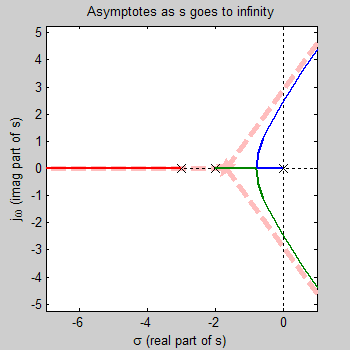
\includegraphics[width=\linewidth]{asymp1.png}
    \caption{Pour $\frac{1}{s(s^2+5s+6)}$.
    Les asymptotes partent de $\frac{-3-2+0}{3} \approx -1.67$.}
    \label{fig:asymp1}
  \end{subfigure}
  \begin{subfigure}{0.49\linewidth}
    \centering
    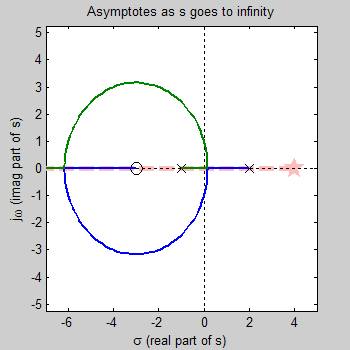
\includegraphics[width=\linewidth]{asymp2.png}
    \caption{Pour $\frac{s+3}{s^2-s-2}$.
    L'asymptote part de $\frac{-1+2-(-3)}{1} = 4$.}
    \label{fig:asymp2}
  \end{subfigure}
  \caption{Asymptotes vers lequels $n-m$ pôles partent.
  Images prisent de \cite{cheever2013rlocus}.}
  \label{fig:asymp}
\end{figure}

\subsection{Méthode de dessin à la main}
C'est très facile à dessiner à la main.
On part pour $k = 0$ des $n$ pôles et on trace $n$ courbes qui sont les évolutions des racines du
polynôme caractéristique en fonction de $k$.

Supposons qu'on ait que des racines et pôles réels,
on part donc de ces racines et pôles et on essaie de rester le plus possible sur l'axe réel et essayer
de rejoindre un zéro ou une asymptote.
On saut aussi que pour n'importe quel cas, on aura jamais de racine à gauche d'un nombre \emph{pair}
de zéro ou de pôle.
Les zones autorisées sont représentées par la \figuref{locus1} et la \figuref{locus2}.

\begin{figure}
  \begin{subfigure}{0.49\linewidth}
    \centering
    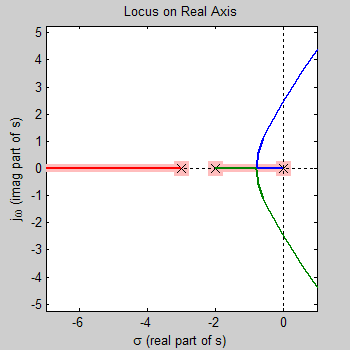
\includegraphics[width=\linewidth]{locus1.png}
    \caption{Pour $\frac{1}{s(s^2+5s+6)}$.}
    \label{fig:locus1}
  \end{subfigure}
  \begin{subfigure}{0.49\linewidth}
    \centering
    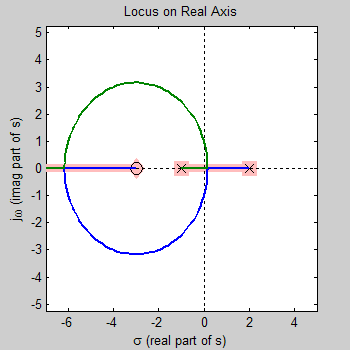
\includegraphics[width=\linewidth]{locus2.png}
    \caption{Pour $\frac{s+3}{s^2-s-2}$.}
    \label{fig:locus2}
  \end{subfigure}
  \caption{Zônes où le polynôme caractéristique peut avoir des racines.
  Images prisent de \cite{cheever2013rlocus}.}
  \label{fig:locus}
\end{figure}

On voit avec la \figuref{locus2} que ça complique la tâche car il faut faire un détour.
Les points où on quitte l'axe réel ou qu'on rejoint l'axe réel sont des solutions (réelles évidemment) de
\[ N(s)D'(s) - N'(s)D(s) = 0. \]

\begin{myexem}
  Pour $\frac{1}{s(s^2+5s+6)}$, on part des 3 pôles $-2$, $-3$ et 0.
  Il n'y a pas de zéro et les asymptotes sont données par la \figuref{asymp1}.
  $-3$ part vers la gauche et les deux autres vers la droite car c'est là
  qu'ils sont autorisés à aller (voir la \figuref{locus1}).
  Le pôle en $-3$ prend alors simplement l'asymptote à \ang{180}.
  Pour savoir où les deux autres se sépare, on analyse
  \[ N(s)D'(s) - N'(s)D(s) = 3s^2+10s+6 \]
  qui a comme racine $\frac{-5\pm\sqrt{7}}{3}$ mais $\frac{-5-\sqrt{7}}{3}$ est entre $-3$ et $-2$
  et n'est donc pas autorisé (voir la \figuref{locus1}).
  Ils se recontrent donc en $\frac{-5+\sqrt{7}}{3}$ puis se séparent.
  Un va vers l'asymptote en \ang{60}, l'autre en \ang{-60},
  ça n'a pas de sens de demander lequel va où.
\end{myexem}
\begin{myexem}
  Pour $\frac{s+3}{s^2-s-2}$, on a 2 pôles $-1$ et 2 et un zéro $-3$.
  Il y a donc $2-1 = 1$ asymptote qui est donnée par la \figuref{asymp2}.
  \figuref{locus2} nous permet de voir que $-1$ par vers la droite et 2 vers la gauche.
  Pour savoir où ils se séparent et où ils se rejoignent, on résoud
  \[ N(s)D'(s) - N'(s)D(s) = (s+3)(2s-1) - (s^2-s-2) = s^2+6s-1 = (s-(-3+\sqrt{10}))(s-(-3-\sqrt{10})). \]
  Ils se séparent donc en $-3+\sqrt{10}$ et se rejoignent en $-3-\sqrt{10}$.
  Ensuite, l'un va vers $-3$ et l'autre vers l'axymptote à \ang{180}.
  La question de savoir qui va où n'a pas de sens.

  On voit ici que comme $C_0(s)G(s)$ est instable,
  le raisonnement qu'on a fait ne s'applique plus et augmenter $k$ stabilise le système.
\end{myexem}

\section{Robustesse}
C'est bien qu'un système soit stable mais on est jamais à l'abris d'une erreur de
modélisation ou d'une non-linéarité.
Il vaut donc mieux ne pas être tout juste table mais avoir une certaine marge.

Il y a 4 marges différentes, avec $p_i$ les pôles de $1 + C(s)G(s)$,
\begin{align*}
  & \text{Marge de stabilité} & \sigma_R & = -\max \Re(p_i)\\
  & \text{Marge absolue de stabilité}  & \sigma_M & = \inf_\omega|1 + C(j\omega)G(j\omega)|\\
  & \text{Marge de phase}  & \phi_M & = \arg(C(j\omega)(G(j\omega)) + \ang{180}\\
  & \text{Marge de gain}  & G_M & = 1 - |C(j\omega_L)G(j\omega_L)|
\end{align*}
où $\arg:\R\to[-\ang{360};0]$.

Il est aisé de vérifier qu'on respecte une marge de robustesse $\sigma_R$.
Il suffit de regarder si $1 + C(s')G(s')$ est stable où $s' = s + \sigma_R$.
On remplace donc simplement les $s$ par $s' - \sigma_R$ dans l'expression
et on utilise les critères des stabilités normaux
(Routh-Hurwirz, Nyquist, Bode, ...).

\begin{figure}
  \begin{subfigure}{0.49\linewidth}
    \centering
    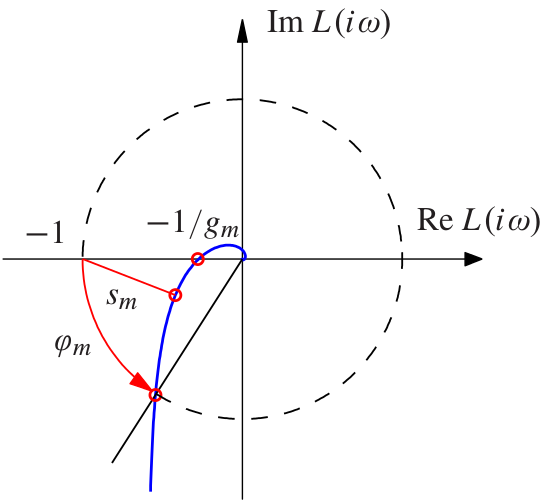
\includegraphics{nyquist-robust.png}
    \caption{$\sigma_M$, $\phi_M$ et $G_M$ dans le diagramme de Nyquist.}
    \label{fig:nyquist-robust}
  \end{subfigure}
  \begin{subfigure}{0.49\linewidth}
    \centering
    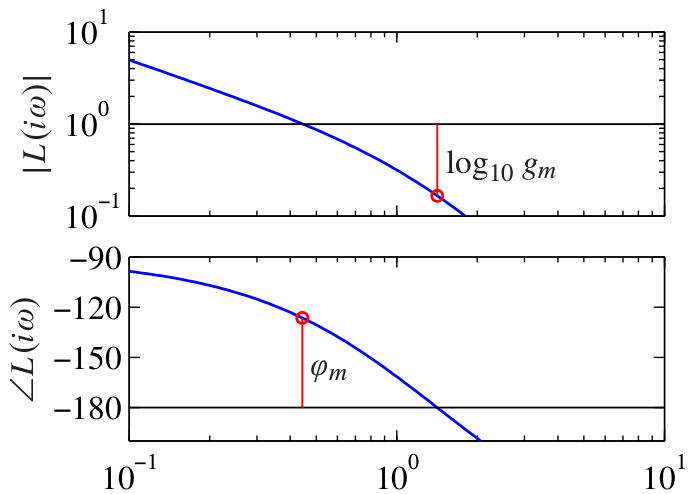
\includegraphics{bode-robust.png}
    \caption{$\phi_M$ et $G_M$ dans le diagramme de Bode.}
    \label{fig:bode-robust}
  \end{subfigure}
  \caption{Marges dans Nyquist et Bode avec $s_m$ pour $\sigma_M$,
  $\varphi_m$ pour $\phi_M$ et $g_m$ pour $G_M$ \cite{astrom2010feedback}.}
  \label{fig:robust-graph}
\end{figure}

$\sigma_M$, $\phi_M$ et $G_M$ peuvent être obtenu à l'aide
du diagramme de Bode et de Nyquist comme illustré à la \figuref{robust-graph}.

Ils peuvent également s'obtenir via identification à la fonction
de transfert de référence
\[ T_r(s) = \frac{\omega_n^2}{s^2 + 2 \zeta \omega_n s + \omega_n^2}. \]
On a
\[ \sigma_M = \inf_\omega \left|1 + C(j\omega)G(j\omega)\right| =
\inf_\omega \sqrt{1 + \frac{1 - 2\left(\frac{\omega}{\omega_n}\right)^2}{\left(\frac{\omega}{\omega_n}\right)^4 + 4\zeta^2\left(\frac{\omega}{\omega_n}\right)^2}} \]
$\sigma_M$ est atteint pour
\[ \left(\frac{\omega}{\omega_n}\right)^2 = \frac{1 + \sqrt{1 + 8\zeta^2}}{2}. \]
$\sigma_M$ ne dépend donc que de $\zeta$ et
\[ \sigma_M^2 = 1 - \frac{4\sqrt{8\zeta^2+1}}{(8\zeta^2+1)^{3/2}+\sqrt{8\zeta^2+1}+16\zeta^2+2}. \]

De plus,
\begin{align*}
  \frac{\omega_c}{\omega_n} & = \sqrt{\sqrt{4\zeta^4 + 1} - 2\zeta^2}\\
  \phi_M & = \arctan\left(\frac{2\zeta}{\frac{\omega_c}{\omega_n}}\right)
\end{align*}

\subsection{Sensibilité}
On analyse la sensibilité normalisée.
Par exemple, pour la sensibilité de $T_v$ par rapport à $H$,
ce n'est pas juste $\fdif{T_V}{H}$ mais
\[ S_v = \fdif{T_v}{H} \frac{H}{T_v} = \frac{1}{(1 + CG)^2}\frac{H}{\frac{H}{1+CG}} = \frac{1}{1+CG}. \]
On remarque qu'on a aussi
\[ \sigma_M^{-1} = \sup_\omega\frac{1}{|1+C(j\omega)G(j\omega)|}
= \sup_\omega |S_v(j\omega)|. \]
On voit bien dans la \figuref{nyquist-robust},
qu'il est difficile d'avoir $\sigma_M > 1$, on essaie donc d'avoir $\sigma_M$
le plus grand possible tout en restant réaliste donc avoir $\sigma_M$ le plus proche
de 1 tout en restant $< 1$.
On essaie donc d'avoir $\sigma_M^{-1}$ le plus proche de 1 tout en restant $> 1$.
Dans la \figuref{sensitivity}, on veut donc que $|S_v|$ dépasse le moins possible
au dessus de 1 (à ne pas confondre avec le dépassement $D$ qui se mesure sur la réponse
à un échelon).

On aime aussi être peu sensible à une large bande en basse fréquence.
Ce gabarit est aussi illustré par la \figuref{sensitivity}.

Seulement, on sait aussi,
par le théorème de Bode\cite[p.~336]{astrom2010feedback}
que que si le degré relatif de $C(s)G(t)$ $\geq 2$,
\[ \int_0^\infty \ln|S_v(j\omega) \dif \omega = \pi \sum_k \Re(p_k) \]
où $p_k$ sont les pôles \emph{instables} de $C(s)G(s)$.
S'ils n'en ont pas, l'intégrale vaut donc 0.

\begin{figure}
  \begin{subfigure}{0.3\linewidth}
    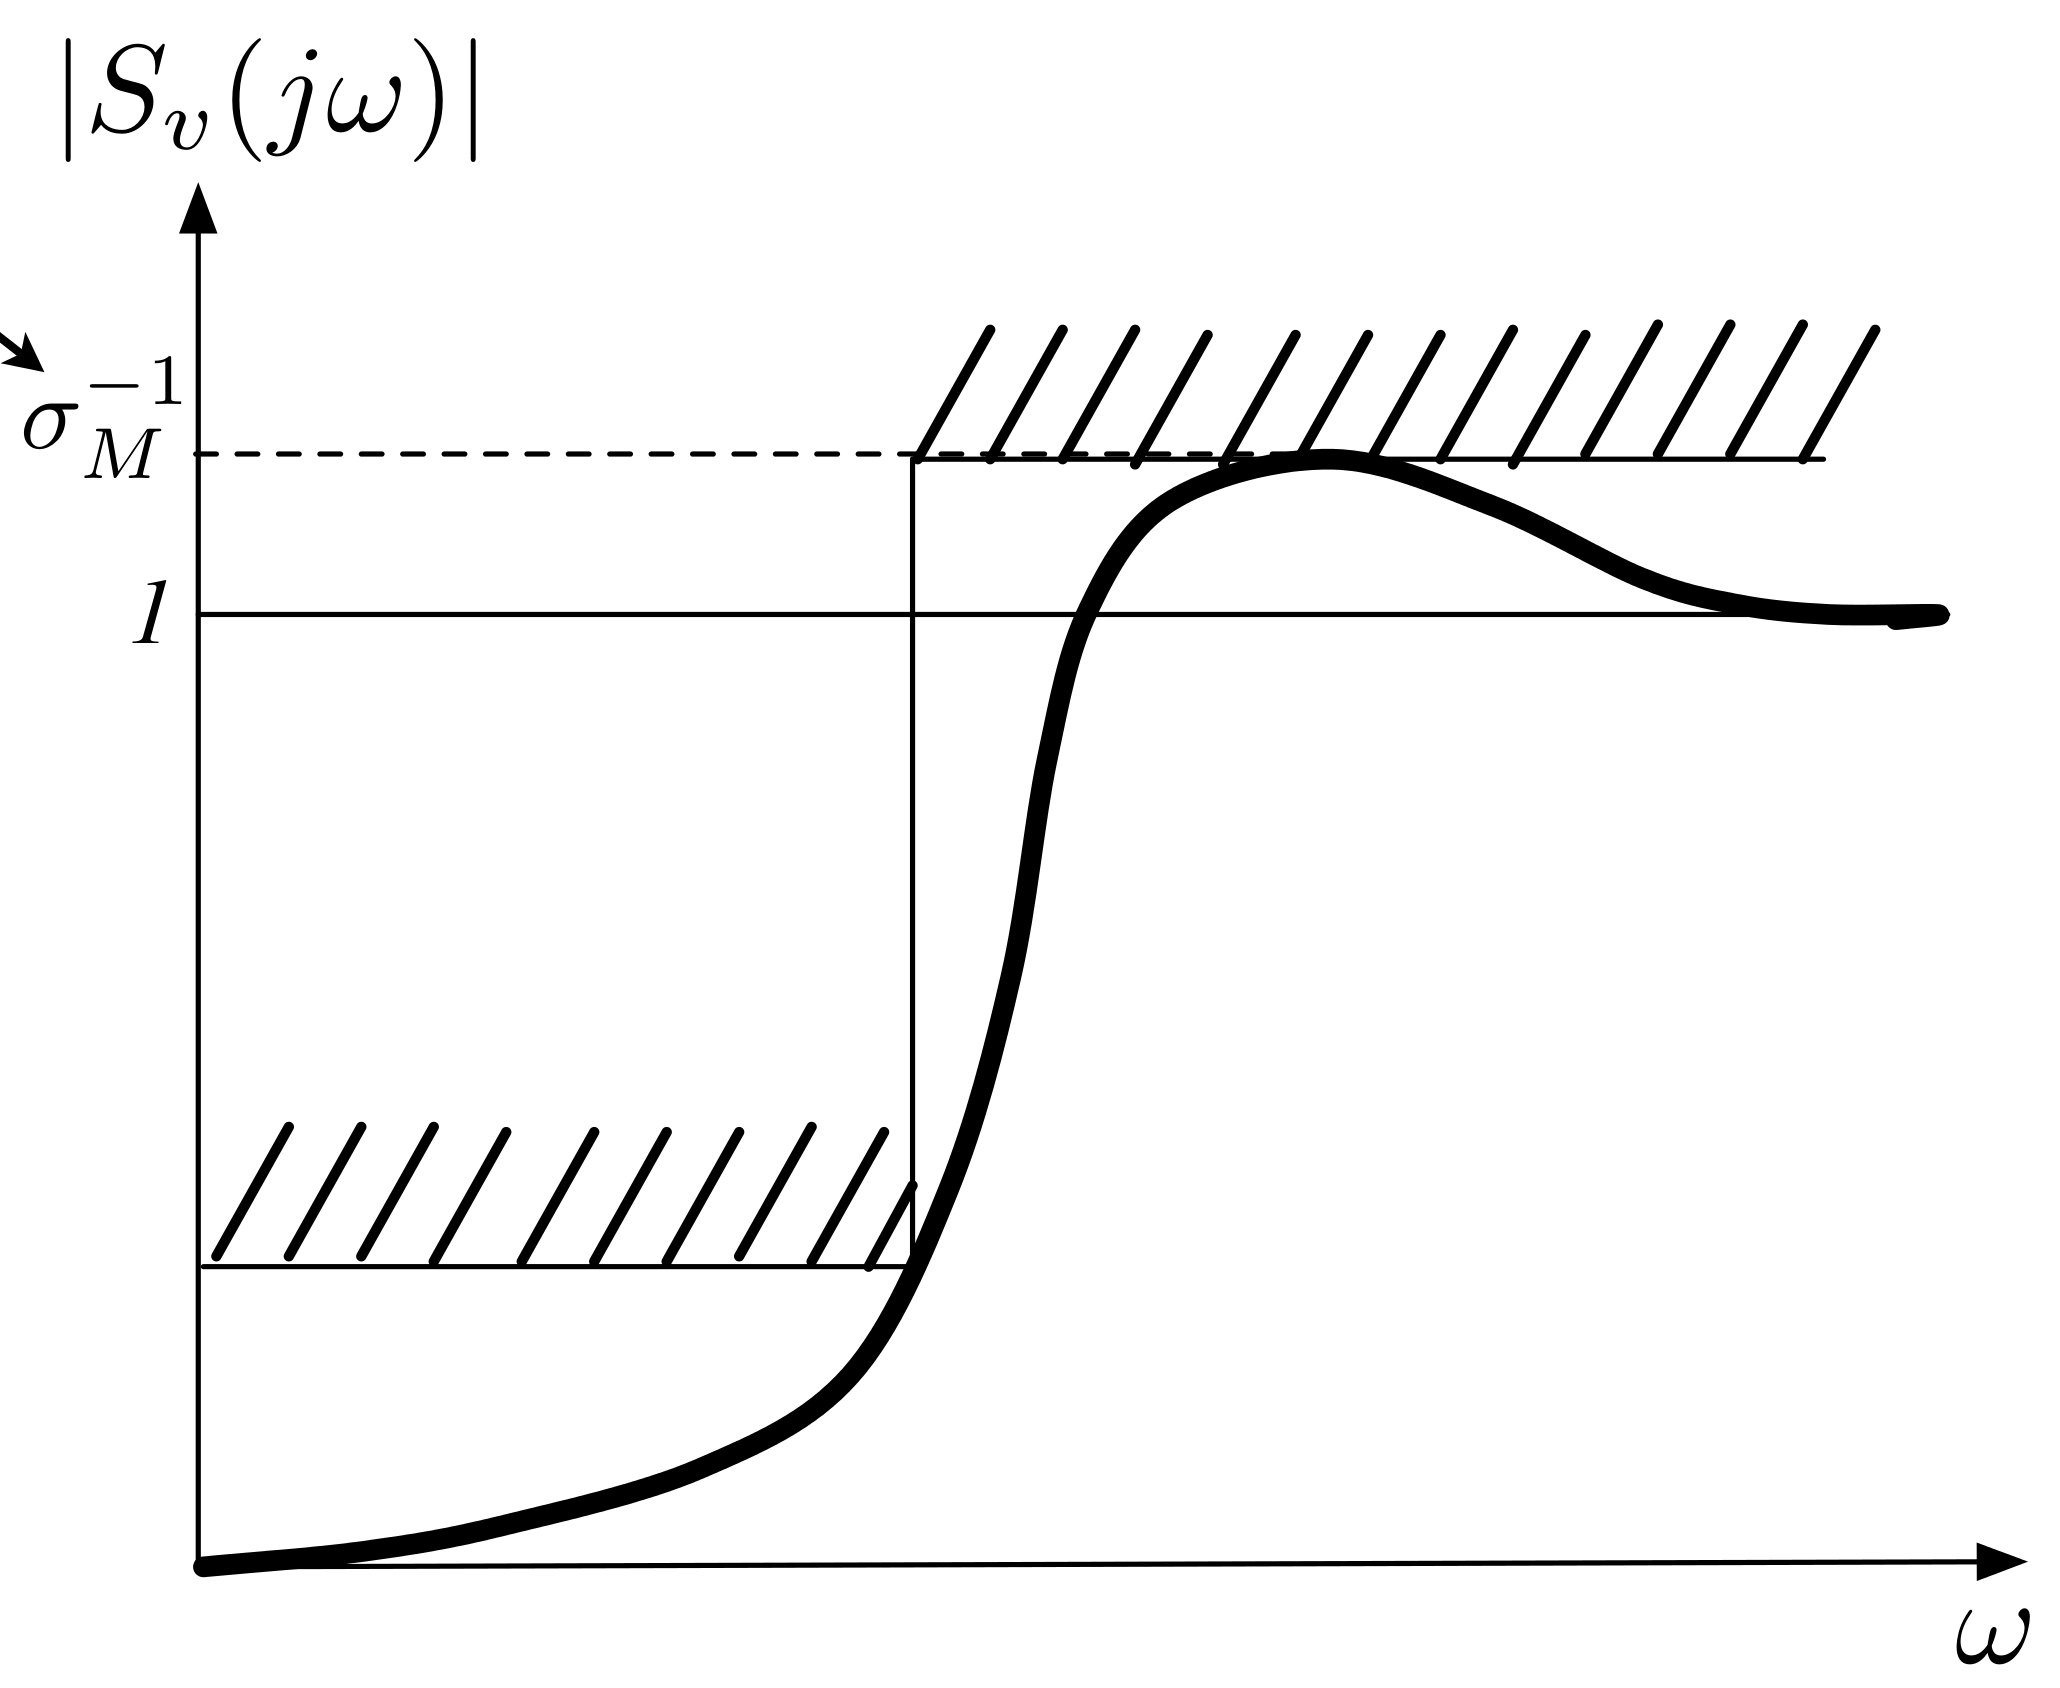
\includegraphics[width=\linewidth]{sensitivity.png}
    \caption{Gabarits pour $S_v$.
    Rappelons qu'avec une action intégrale,
    $|C(j0)G(j0)| \to \infty$ et $C(j\infty)G(j\infty)| = 0$
    ce qui explique la forme de $|S_v(s)| = \frac{1}{|1+C(s)G(s)|}$.}
    \label{fig:sensitivity}
  \end{subfigure}
  \begin{subfigure}{0.3\linewidth}
    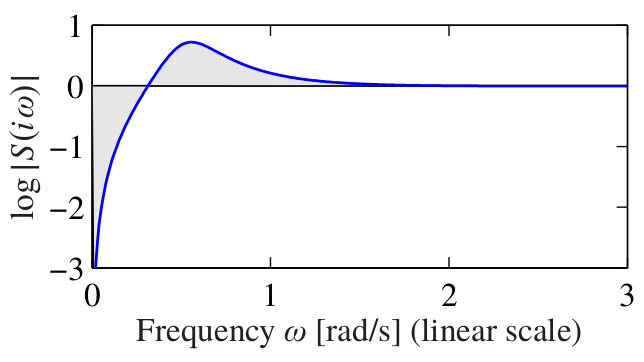
\includegraphics[width=\linewidth]{sensitivity-log.png}
    \caption{$S_v$ en échèle semi-logarithmique avec
    l'intégrale du théorème de Bode colorée\cite{astrom2010feedback}.}
    \label{fig:sensitivity-log}
  \end{subfigure}
  \begin{subfigure}{0.3\linewidth}
    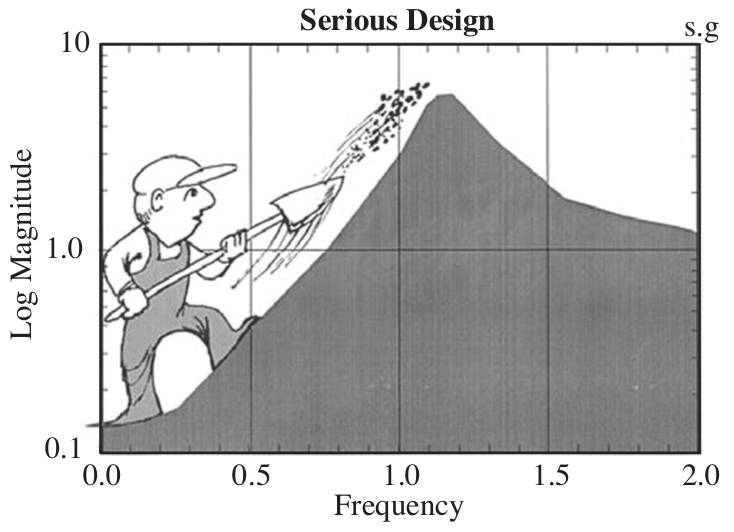
\includegraphics[width=\linewidth]{sensitivity-shovel.png}
    \caption{Le compromis entre nos deux gabarits qu'on doit faire
    à cause du théorème de Bode illustré\cite{astrom2010feedback}.}
    \label{fig:sensitivity-shovel}
  \end{subfigure}
  \caption{Illustration du lien entre le théorème de Bode
  et les gabarits sur $S_v$.}
\end{figure}

Seulement, comme on le voit en comparant la \figuref{sensitivity} et la \figuref{sensitivity-log}
que si on veut être peu sensible à une large bande en basse fréquence et avoir un $\sigma_M^{-1}$ proche de 1,
on aura une intégrale très négative.
Ce n'est pas possible par le théorème de Bode et c'est encore pire si on a des pôles instables.
En essayant de diminuer notre sensibilité aux basses fréquences ou d'augmenter la bande
de basse fréquence où on est peu sensible, on augmentera donc $\sigma_M^{-1}$
et vice-versa.
En voyant ça de façon imagée à l'aide de la \figuref{sensitivity-shovel},
on veut faire un trou large et profond sans avoir un tas de terre trop haut à côté.

Bien étaller le tas de terre serait bien évidemment une solution mais je doute que ce soit évident.

\section{Régulateur PID}
En se rappelant de Laplace, on peut donner un sens plus intuitif à notre régulation.
Que faisons-nous avec l'erreur ?
\begin{itemize}
  \item Si $C(s) = 1$, on met simplement $u$ à l'erreur.
  \item Si $C(s) = \frac{1}{s}$,
    $U(s) = \frac{E(s)}{s}$ donc $u(t) = \int_{-\infty}^t e(\tau) \dif \tau$.
    $u(t)$ est donc l'intégrale de l'erreur.
  \item Si $C(s) = s$,
    $U(s) = sE(s)$ donc $u(t) = \fdif{e(t)}{t}$.
    $u(t)$ est donc la dérivée de l'erreur.
\end{itemize}
Voyons voir l'intérêt de chacun de ces effets.

\subsection{Régulateur P}
Supposons qu'on ait uniquement une action proportionnelle,
n'est-ce pas suffisant ?
Je pense que la première fois qu'on arrive devant un problème de régulation,
le premier réflexe est de penser à une action proportionnelle et de penser que ça va marcher.
Il faut cependant bien voir que $C(s)E(s)$ ne va pas être la modification qu'on va faire
à $u(t)$ mais bien directement la valeur de $u(t)$ !
Supposons un système trivial où $G(s) = 2$.
Avec $C(s) = k_p$, on va arrêter de changer $u(t)$ lorsque
$u(t) = k_p(2u(t) - r)$, c'est donc lorsque
$u(t) = \frac{rk_p}{1 - 2k_p}$.
On aura donc $y = r\frac{2k_p}{1+2k_p}=rT_r(s)$ qui ne vaut
jamais $r$.

On va donc s'arrêter, soit-disant satisfait avec notre $u(t)$,
alors qu'on a même pas le bon $y(t)$.
En fait l'action proportionnelle est surtout bonne avec un $G(s)$
avec de l'intégrale sous le capot !
En effet, si $y(t)$ intègre $u(t)$, alors ça a du sens de mettre
du $u(t)$ négatif si on est $y(t)$ est trop grand et du positif
si $y(t)$ est trop petit.

Mais si $G(s)$ n'a pas une intégrale pure $\frac{1}{s}$, on aura
une erreur statique comme on le voit sur la \figuref{proportionnal}.

En résumé, une action proportionnelle est bête mais tout de même
importante parmis les trois action PID.
C'est un peu Sid.

\begin{figure}
  \begin{subfigure}{0.3\linewidth}
    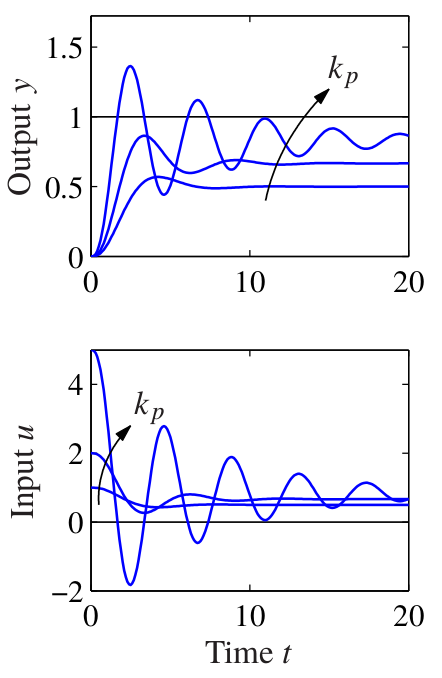
\includegraphics[width=\linewidth]{proportionnal.png}
    \caption{Régulateur P\cite{astrom2010feedback}.}
    \label{fig:proportionnal}
  \end{subfigure}
  \begin{subfigure}{0.3\linewidth}
    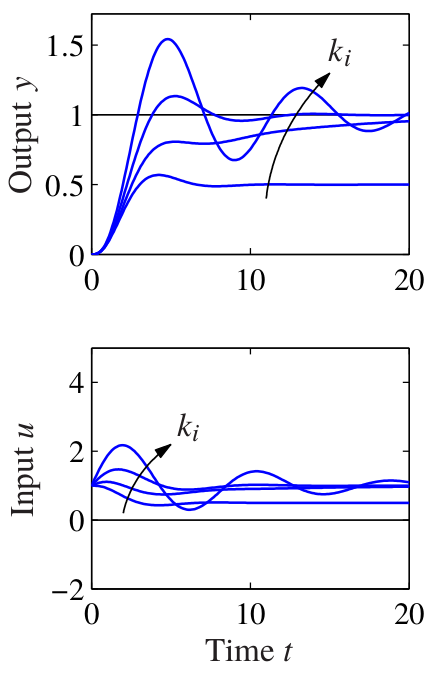
\includegraphics[width=\linewidth]{pi.png}
    \caption{Régulateur PI\cite{astrom2010feedback}.}
    \label{fig:pi}
  \end{subfigure}
  \begin{subfigure}{0.3\linewidth}
    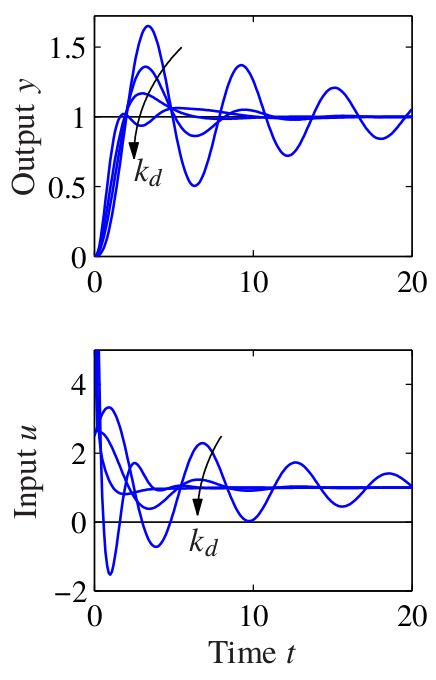
\includegraphics[width=\linewidth]{pid.png}
    \caption{Régulateur PID\cite{astrom2010feedback}.}
    \label{fig:pid}
  \end{subfigure}
  \caption{Illustration de l'utilité de chaque composante
  d'un régulateur PID.}
\end{figure}

\subsection{Régulateur PI.}
Un régulateur PI applique une action intégrale en \emph{parallèle} à l'action
proportionnelle.
On a donc $C(s) = k_p + \frac{k_i}{s}$ et \emph{non} $\frac{k_pk_i}{s}$.
On aura donc deux actions qui auront chacune la parole et dicteront à $u(t)$ ce
qu'il doit faire. Ce dernier les écoutera tous les deux et appliquera la somme
de leur commande, pondérées par $k_p$ et $k_i$.

L'avantage de l'action intégrale, c'est qu'on sait que quand $u(t)$ ne bouge plus,
c'est qu'on a arrêté d'intégrer et donc que l'erreur est nulle car on intègre l'erreur.
C'est donc la mémoire du régulateur, qui permet donc, avec de bon paramètres $k_p$ et $k_i$
d'avoir un régulateur un peu plus intelligent.

On voit sur la \figuref{pi} qu'on a maintenant plus d'erreur statique grâce à l'action
intégrale.

\subsection{Régulateur PID.}
Le problème c'est qu'on a maintenant pas mal de dépassement car lorsque $y$ s'approche de $r$
et donc que l'erreur s'approche de 0, bien que l'action proporitonnelle est moins grande
(mais est toujours dans le même sens), l'action intégrale continue plein gaz.

Une dérivée verrait que l'erreur diminie bien vite et donnerait donc un ordre contraire
à l'intégrale, pour permettre d'anticiper et de réduire de dépassement.
On voit en effet sur la \figuref{pid} que l'action dérivée diminue le dépassement.

L'action proportionnelle est donc bête mais importante,
l'action intégrale est le sage de la bande qui grâce à sa mémoire et à sa vision
long terme permet d'avoir un errer statique nulle et
l'action dérivée permet d'avoir un peu d'anticipation et donc d'efficacité.

La meilleur image de ce trio est le trio de ``Ice Age'' où Sid joue le rôle de l'action
proportionnelle, Manny l'action intégrale et Diego l'action dérivée.

\section{Emballement}

\begin{figure}[!ht]
  \centering
  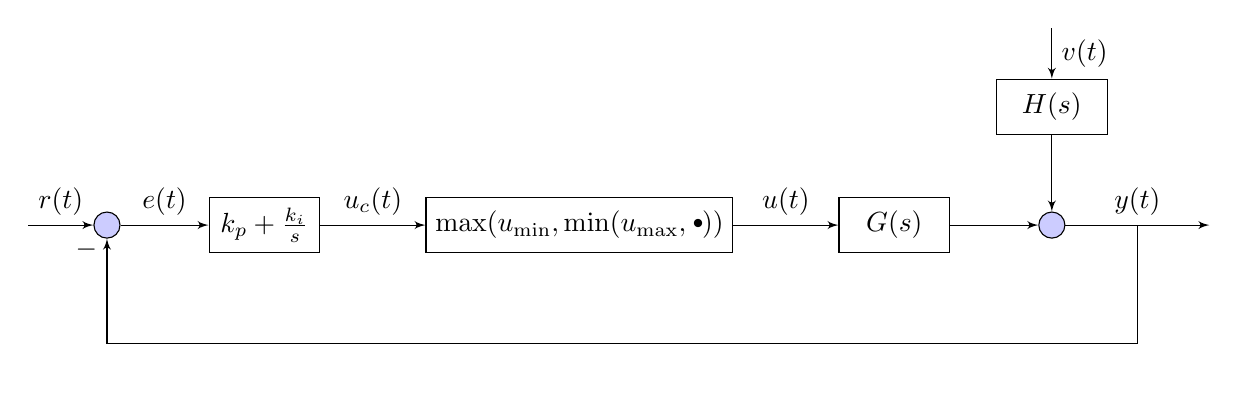
\begin{tikzpicture}[auto, node distance=2cm,>=latex']
    \node [input, name=input] {};
    \node [sum, right of=input] (sum) {};
    \node [block, right of=sum, node distance=2cm] (C) {$k_p + \frac{k_i}{s}$};
    \node [block, right of=C, node distance=4cm] (S) {$\max(\umin,\min(\umax,\sbt))$};
    \node [block, right of=S, node distance=4cm] (G) {$G(s)$};
    \node [sum, right of=G, node distance=2cm] (sum2) {};
    \node [block, above of=sum2, node distance=1.5cm] (H) {$H(s)$};
    \node [input, above of=H, name=pert, node distance=1cm] {};
    \node [output, right of=sum2] (output) {};
    \node [below of=S] (feedback) {};
    \draw [->] (input) -- node {$r(t)$} (sum);
    \draw [->] (pert) -- node {$v(t)$} (H);
    \draw [->] (H) -- (sum2);
    \draw [->] (C) -- node {$u_c(t)$} (S);
    \draw [->] (S) -- node {$u(t)$} (G);
    \draw [->] (sum) -- node {$e(t)$} (C);
    \draw [->] (G) -- (sum2);
    \draw [->] (sum2) -- node[name=y] {$y(t)$} (output);
    \draw (y) |- ($(S)+(0,-1.5cm)$);
    \draw [->] ($(S)+(0,-1.5cm)$) -| node[pos=0.95] {$-$} (sum);
  \end{tikzpicture}
  \caption{Schéma-block d'un système avec saturation.}
  \label{fig:windup-block}
\end{figure}

Toute notre analyse se base sur le fait que nous avons des systèmse LTI (Linear Time Invariant).
Pourtant, en pratique, il y a pas mal de cause de non-linéaire.
Une assez courante est la \emph{saturation} de la commande.
Ça a lieu lorsque le système ne sait qu'appliquer une commande entre $\umin$ et $\umax$.
On modélise alors notre système avec une composante non-linéaire appelée saturation.
Son entrée est la commande voulue $u_c$ et sa sortie la commande vraiment appliquée $u$.
On a la relation $u = \min(\umax, \max(\umin, u_c))$, c'est à dire que si $u_c \geq \umax$,
on prend $u = \umax$ et si $u_c \leq \umin$, on prend $u = \umin$, sinon on a $u = u_c$.
Le système est représenté par la \figuref{windup-block}.

Comme la composante de saturation est non-linéaire on ne peut plus représenter cette composante
par une convolution en temporelle ou un produit en fréquentiel et on ne peut donc faire d'analyse
fréquentielle.

\begin{figure}
  \centering
  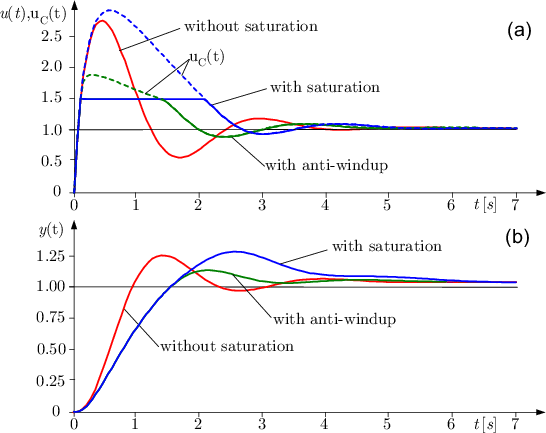
\includegraphics[width=0.6\linewidth]{schmidwindup.png}
  \caption{Exemple de l'application d'un système anti-emballement pris de~\cite{schmid2005windup}.
  La courbe rouge montre le comportement du système sans saturation.
  On rajoute une saturation à \num{1.5} pour la courbe bleue.
  La courbe verte a la saturation et le système emballement.}
  \label{fig:schmidwindup}
\end{figure}

Dans la \figuref{schmidwindup}, on voit que sans la saturation,
on arrive plus vite à la consigne.
Avec la saturation, $u$ n'est pas aussi grand qu'on aimerait et on va donc
moins vite.
Cette lenteur fait que l'intégrale a plus le temps de gonfler.
En effet, on voit que l'aire entre la consigne 1 et la courbe rouge dans
le graphe de $y$ est plus petite que celle entre la consigne et la courbe bleue.
Lorsqu'on atteint la consigne, l'intégrale est donc plus grosse pour le système
avec saturation.
Il va donc prendre beaucoup plus de temps à réaliser qu'il faut redescendre
et l'intégrale risque d'à nouveau trop gonfler.

\begin{figure}
  \centering
  \begin{subfigure}{0.49\linewidth}
    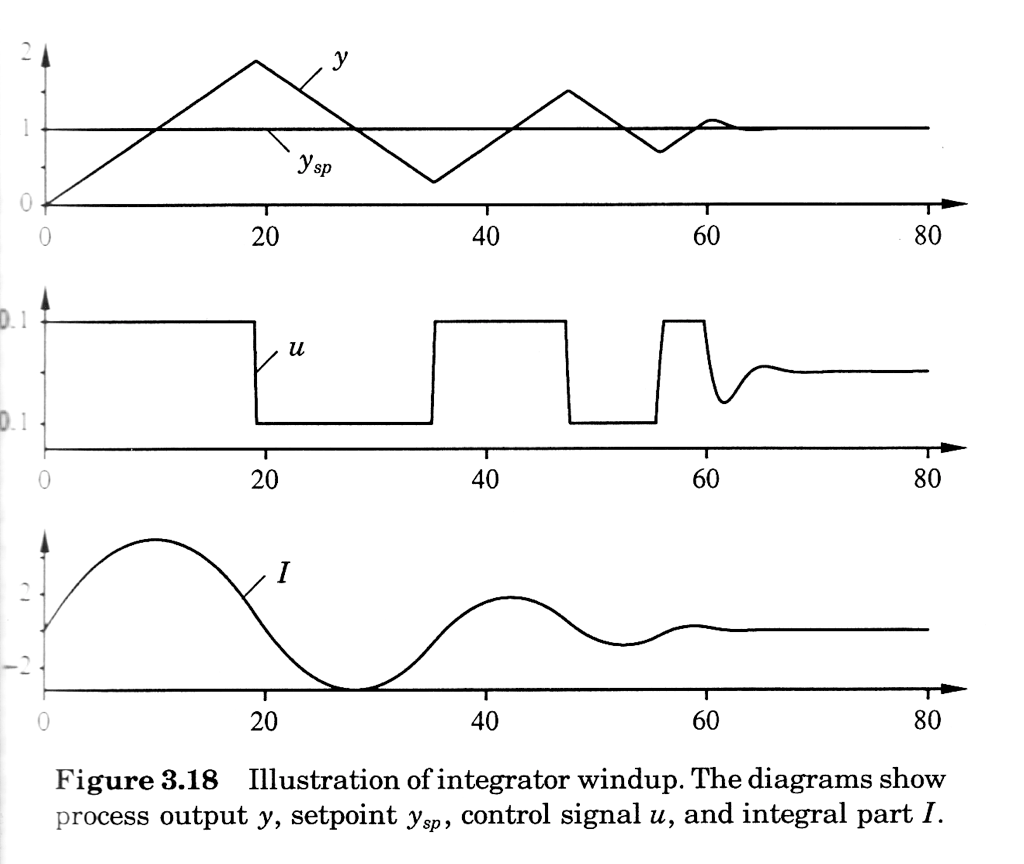
\includegraphics[width=\linewidth]{windup.png}
    \caption{Exemple d'emballement.}
    \label{fig:windup}
  \end{subfigure}
  \begin{subfigure}{0.49\linewidth}
    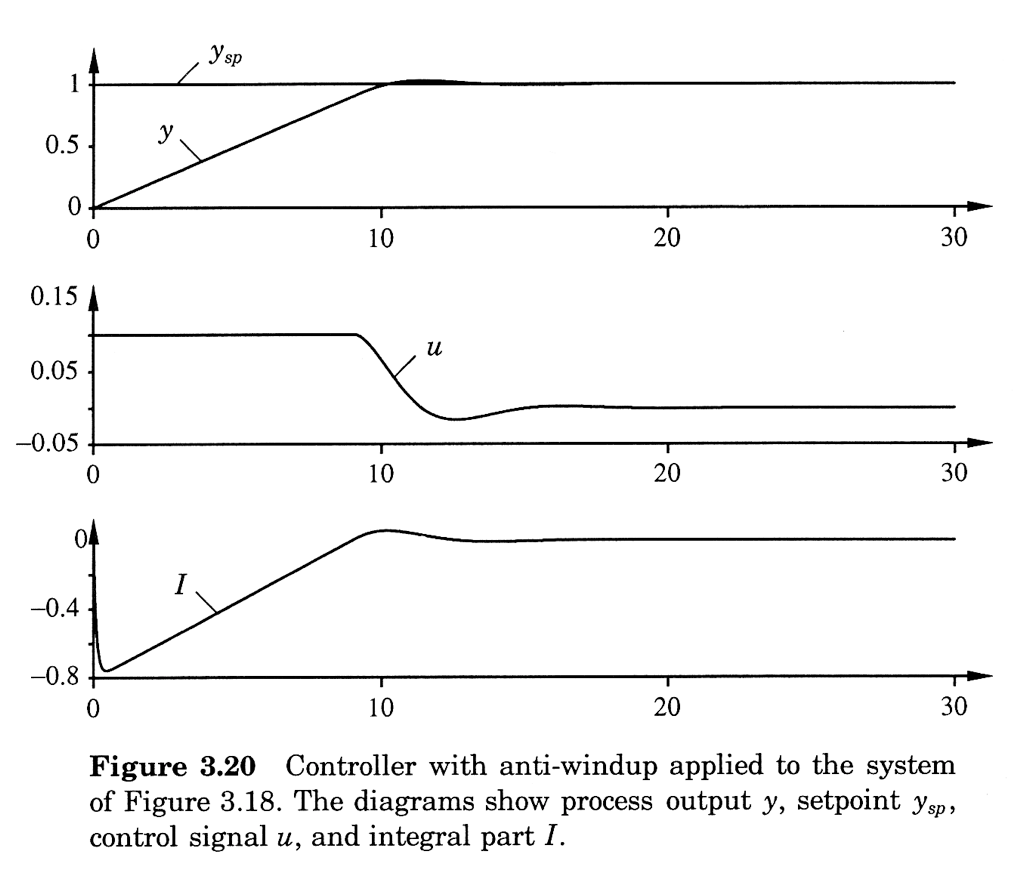
\includegraphics[width=\linewidth]{anti-windup.png}
    \caption{Application d'un système anti-emballement à l'exemple de la \figuref{windup}.}
    \label{fig:anti-windup}
  \end{subfigure}
  \caption{Exemple d'emballement avec application d'un système anti-emballement.}
  \label{fig:windup-cm}
\end{figure}

Il arrive qu'il prenne tellement de temps à s'en rendre compte, c'est à dire
que l'intégrale prend tellement de temps à dégonfler que l'erreur est très
grande lorsque l'intégrale est enfin nulle se qui fait qu'on atteint l'autre borne
pour de la commande très rapidement.
On est alors reparti pour un tour.
C'est ce qu'on observe à la \figuref{windup} en $t = 19$,
dans le graphe de $u$, on passe tellement vite d'une borne à l'autre qu'on a l'impression
que c'est un point de discontinuité.
On voit en effet, en regardant le graphe pour $y$ à $t = 19$ qu'on avait atteint une erreur
assez importante.

\subsection{Système anti-emballement}

\begin{figure}[!ht]
  \centering
  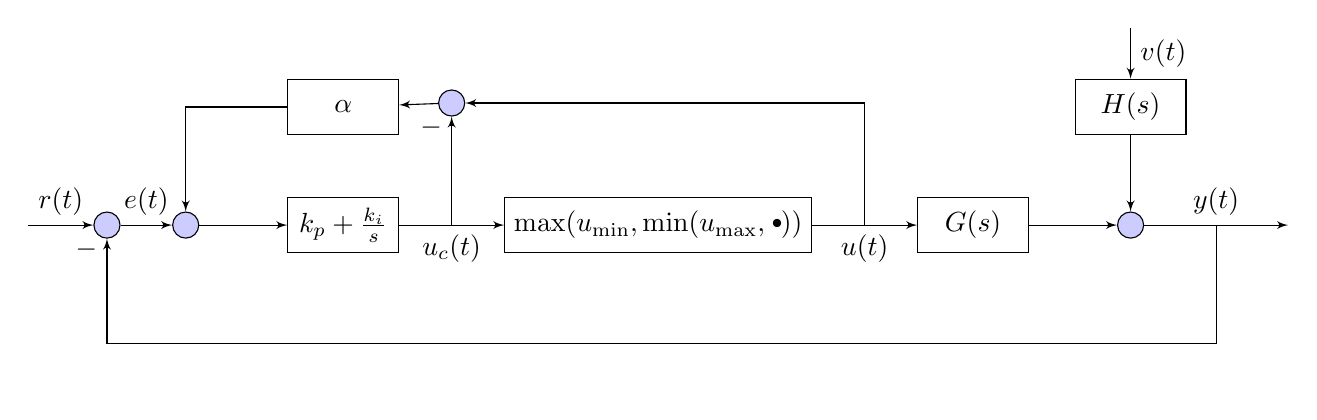
\begin{tikzpicture}[auto, node distance=2cm,>=latex']
    \node [input, name=input] {};
    \node [sum, right of=input] (sum) {};
    \node [sum, right of=sum] (sum4) {};
    \node [block, right of=sum4, node distance=2cm] (C) {$k_p + \frac{k_i}{s}$};
    \node [block, right of=C, node distance=4cm] (S) {$\max(\umin,\min(\umax,\sbt))$};
    \node [block, right of=S, node distance=4cm] (G) {$G(s)$};
    \node [sum, right of=G, node distance=2cm] (sum2) {};
    \node [block, above of=sum2, node distance=1.5cm] (H) {$H(s)$};
    \node [input, above of=H, name=pert, node distance=1cm] {};
    \node [output, right of=sum2] (output) {};
    \node [below of=S] (feedback) {};
    \draw [->] (input) -- node {$r(t)$} (sum);
    \draw [->] (pert) -- node {$v(t)$} (H);
    \draw [->] (H) -- (sum2);
    \draw [->] (C) -- node[below,name=uc] {$u_c(t)$} (S);
    \draw [->] (S) -- node[below,name=u] {$u(t)$} (G);
    \draw [->] (sum) -- node {$e(t)$} (sum4);
    \draw [->] (sum4) -- (C);
    \draw [->] (G) -- (sum2);
    \draw [->] (sum2) -- node[name=y] {$y(t)$} (output);
    \draw (y) |- ($(S)+(0,-1.5cm)$);
    \draw [->] ($(S)+(0,-1.5cm)$) -| node[pos=0.95] {$-$} (sum);

    \node [block, above of=C, node distance=1.5cm] (a) {$\alpha$};
    \node [sum, above of=uc, node distance=1.85cm] (sum3) {};
    \draw [->] (sum3) -- (a);
    \draw [->] (uc) -- node[pos=0.9] {$-$} (sum3);
    \draw [->] (u) |- (sum3);
    \draw [->] (a) -| (sum4);
  \end{tikzpicture}
  \caption{Schéma-block d'un système avec saturation et système anti-emballement.}
  \label{fig:anti-windup-block}
\end{figure}

On voit que les problèmes d'emballement sont liés à la composantes intégrale.
Il nous faut alors, pour remédier à l'emballement, ajouter un système qui détectera quand
$u_c \geq u$, c'est à dire que $u_c \geq \umax$ ou $u_c \leq u$, c'est à dire $u_c \leq \umin$,
et qui videra l'intégrale qui est trop positive ou trop négative.
Un système anti-emballement classique est représenté par la \figuref{anti-windup-block}.

\begin{itemize}
  \item Si $u = u_c$, ce système n'a aucun effet car $u - u_c = 0$.
  \item Si $u \leq u_c$, ça peut signifier 2 choses
    \begin{description}
      \item[Une trop grosse action proportionnelle]
        L'erreur est très grande par rapport à $\umax$, ou plus précisément que $k_p e(t) \gg \umax$,
        on va donc être trop lent pour arriver à $e(t) = 0$ et on va donc intégrer plus que voulu.
        $u - u_c$ est négatif, avec $e + \alpha (u-u_c)$ comme entrée à $C(s)$,
        on aura toujours $\umax \leq u_c$\footnote{même si $\alpha$ est grand, on ne peut pas avoir $u_c < \umax$ car alors $u = u_c$ et on et donc il n'y a plus que $e$ à l'entrée de $C(s)$ et donc $\umax \leq u_c$.}
        mais on intégrera $e + \alpha (u-u_c) < e$, même si on intégrera plus longtemps que sans la saturation, on intégrera moins,
        l'intégrale sera alors moins gonflée lorsqu'on aura $e(t) = 0$.
      \item[Une trop grosse action intégrale]
        L'erreur n'est plus spécialement grande, elle est même peut-être déjà devenue négative mais
        on continue à vouloir $u_c \geq \umax$ à cause de l'intégrale qui a beaucoup gonflé.
        Pour la même raison que précédemment, on aura toujours $u_c \geq \umax$,
        l'effet va être donc uniquement dans l'intégrale, on va la vider plus rapidement qu'elle se viderait normalement.
    \end{description}
  \item Si $u \geq u_c$, la discussion est pareille que pour $u \leq u_c$.
\end{itemize}
En résumé, l'action du système va être sur l'intégrale, elle va l'empêcher de trop gonfler et puis va la vider plus rapidement.
Elle ne va cependant agir que lorsque la commande sature et ne va donc pas poser de problème dans les cas où il n'y a pas de risque
d'emballement.
Elle ne va faire \emph{pas} descendre $u_c$ en dessous de $\umax$ ou au dessus de $\umin$ quand on sature,
elle ne va donc \emph{pas} augmenter le temps de réponse.

Illustrons cela avec pour commencer la \figuref{schmidwindup} où on voit que le seul effet du système anti-emballement est lorsqu'on dépasse
$\umax = 1.5$.
On voit en pointillé $u_c$ qui est plus petit que pour a courbe bleue mais qui ne descend pas en dessous de $\umax$ tant que $y(t) \leq r(t)$.
Il est par contre beaucoup plus rapide à passer en dessous de $\umax$ lorsuqe $y(t) \geq r(t)$ ce qui montre bien qu'il a empêché à l'intégrale de trop gonfler.

Pour la \figuref{anti-windup}, on voit à nouveau que le système anti-emballement ne fait pas passer $u_c$ en dessous de $\umax$.
Au tout début, on voit que l'intégrale intégre quelque chose de très négatif, ça doit être dû au fait qu'au début, on demande un
très grand $u_c$ et donc $\alpha (u_c-u)$ est très négatif.
Par la suite, comme $\alpha(u_c-u)$ est négatif, l'action proportionnelle est moins forte et l'action intégrale est négative donc
$u_c - u$ est moins important, de telle sorte que $e(t) \geq -\alpha (u_c - u)$, on intègre donc du positif et l'intégrale remonte.
Elle monte d'ailleurs beaucoup plus lentement que pour la \figuref{windup} grâce au fait qu'on intègre aussi $\alpha (u_c - u)$ qui
est négatif.
Au final, lors $y(t) \geq r(t)$, l'intégrale est vide et $u$ ne sature plus, on repasse donc dans un système LTI et le système
anti-emballement n'a plus d'effet.

\section{Matlab}
Voici les commandes utiles sous Matlab
\subsection{Calcul de la fonction de transfert}
\begin{description}
  \item[tf] \lstinline|F = tf([10,30],[1,5,6])| représente la fonction de transfert $F(s)=10\frac{s+3}{s^2+5s+6}$.
    J'ai mis $F$ pour montrer que ça peut être aussi bien $G$, que $H$, $T_v$, $T_r$, ...
    Les autres commandes (sauf \lstinline|tf2ss|) on besoin de la fonction de transfert
    dans la forme renvoyée par \lstinline|tf| ou \lstinline|zpk|.
  \item[zpk] \lstinline|F = zpk([-3],[-2,-3],10)| représente la fonction de transfert $F(s) = 10\frac{s+3}{(s+2)(s+3)}$.
  \item[ss2tf] \lstinline|[N,D] = ss2tf(A,B,C,D,iu)| renvoit le numérateur \lstinline|N| et le dénominateur \lstinline|D|
    de la fonction de transfert correspondant au \lstinline|iu|\ieme{} input de l'équation d'état
    \begin{align*}
      \dot{x} & = Ax + Bu\\
      y & = Cx + Du.
    \end{align*}
    En boucle ouverte, leur $u$ vaut
    $\begin{pmatrix}
      u\\v
    \end{pmatrix}$,
    on prend donc \lstinline|iu = 1| pour $G(s)$
    et \lstinline|iu = 2| pou $H(s)$.
    Pour avoir la fonction de transfert dans la bonne
    forme pour utiliser les autres commandes, il faut ensuite faire
    \lstinline|tf(N,D)|.
  \item[tf2ss] \lstinline|[A,B,C,D] = tf2ss(NUM,DEN)| fait l'inverse de \lstinline|ss2tf|.
  \item[series] \lstinline|FG = F*G| ou \lstinline|FG = series(F,G)| construit la fonction de transfert
    de $F(s)G(s)$.
    \begin{center}
      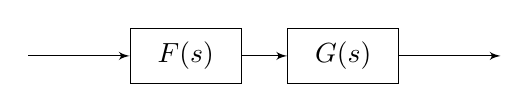
\begin{tikzpicture}[auto,node distance=2cm,>=latex']
        \node [input, name=input] {};
        \node [block, right of=input] (F) {$F(s)$};
        \node [block, right of=F] (G) {$G(s)$};
        \node [output, right of=G] (output) {};
        \draw [->] (input) -- (F);
        \draw [->] (F) -- (G);
        \draw [->] (G) -- (output);
      \end{tikzpicture}
    \end{center}
  \item[parallel] \lstinline|F+G| ou \lstinline|parallel(F,G)| construit la fonction de transfert
    de $F(s) + G(s)$
    \begin{center}
      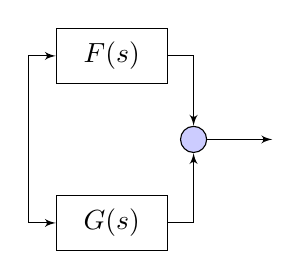
\begin{tikzpicture}[auto,node distance=2cm,>=latex']
        \node [input, name=input] {};
        \node [block, above right of=input, node distance=1.5cm] (F) {$F(s)$};
        \node [block, below right of=input, node distance=1.5cm] (G) {$G(s)$};
        \node [sum, right of=input, node distance=2.1cm] (sum) {};
        \node [output, right of=sum, node distance=1cm] (output) {};
        \draw [->] (input) |- (F);
        \draw [->] (input) |- (G);
        \draw [->] (F) -| (sum);
        \draw [->] (G) -| (sum);
        \draw [->] (sum) -- (output);
      \end{tikzpicture}
    \end{center}
  \item[feedback] \lstinline|feedback(F,G)| construit la fonction de transfert
    de $\frac{F(s)}{1+F(s)G(s)}$.
    \begin{center}
      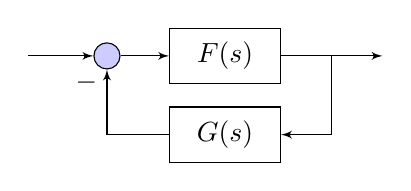
\begin{tikzpicture}[auto,node distance=2cm,>=latex']
        \node [input, name=input] {};
        \node [sum, right of=input] (sum) {};
        \node [block, right of=sum,node distance=1.5cm] (F) {$F(s)$};
        \node [block, below of=F,node distance=1cm] (G) {$G(s)$};
        \node [output, right of=F] (output) {};
        \draw [->] (input) -- (sum);
        \draw [->] (sum) -- (F);
        \draw [->] (G) -| node[pos=0.9] {$-$} (sum);
        \draw [->] (F) -- node (Fr) {} (output);
        \draw [->] (Fr) |- (G);
      \end{tikzpicture}
    \end{center}
    On a par exemple \lstinline|Tr = feedback(series(C,G),1)|.
  \item[pade] \lstinline|[N,D] = pade(T,n)| donne le numérateur \lstinline|N|
    et le dénominateur \lstinline|D| de l'approximation de pade de $e^{-Ts}$ d'ordre
    \lstinline|n|.
    Pour l'appliquer à $F$, il faut ensuite faire \lstinline|tf(N,D)*F|.
\end{description}

\subsection{Analyse de la réponse}
\begin{description}
  \item[step] \lstinline|step(F)| montre le graphe de $y(t) = f * u(t)$,
    c'est à dire la réponse à un échelon.
  \item[impulse] \lstinline|impulse(F)| montre le graphe de $y(t) = f * \delta(t)$,
    c'est à dire la réponse à une impulsion.
  \item[lsim] \lstinline|lsim(F,xt,t)| montre le graphe de $y(t)$ pour une entrée $x(t)$,
    décrite par le vecteur \lstinline|xt| contenant $x(t)$ pour les différents
    temps dans le vecteur \lstinline|t|.
\end{description}

\subsection{Stabilité}
\begin{description}
  \item[nyquist] \lstinline|nyquist(F)| fait le diagramme de Nyquist.
  \item[bode] \lstinline|bode(F)| fait le diagramme de bode.
  \item[rlocus] \lstinline|rlocus(F)| fait le diagramme de root locus.
\end{description}

\subsection{Robustesse}
\begin{description}
  \item[margin] \lstinline|margin(F)| est comme bode mais affiche aussi
    $\omega_c$, $\omega_L$, $\phi_M$, $G_M$ dans le titre du plot dans le format
    ``\lstinline|Gm = |$G_M$\lstinline| (at |$\omega_L$\lstinline|), Pm = |$\phi_M$\lstinline| (at |$\omega_c$\lstinline|)|''.
\end{description}

\subsection{Divers}
\begin{description}
  \item[ltiview] \lstinline|ltiview(F)| lance une GUI avec plusieurs vues
    (on peut choisir ce qui est affiché et combien sont affichées).
    Ça regroupe toutes les autres commandes.
\end{description}

\biblio

\end{document}
